\documentclass{article}

\usepackage{fullpage}
\usepackage{graphicx}
\usepackage{amsfonts, amsmath}
\usepackage{url}
\usepackage{hyperref}
\usepackage{float}
\usepackage[final]{pdfpages}

\hypersetup{
	colorlinks=true,
	linkcolor=black
}

\begin{document}

\clearpage
\vspace*{\stretch{2}}
\begin{center}
\begin{minipage}{.6\textwidth}

\title{Automatic ``Music'' Generator \\ \vspace{2 pt} \text{Final Report}}
\author{Sam Fleckenstein (sef44) \\ Ross Nanopoulos (rdn21)}
\maketitle

\end{minipage}
\end{center}
\vspace{\stretch{3}}
\clearpage

\tableofcontents
\newpage

\section{Abstract}
The purpose of this project is to develop an intelligent music composer that will analyze common and popular patterns in music, reason about those patterns, and generate a new piece of music that is significantly different than the analyzed pieces, while still being interesting.

\newpage

\section{Introduction}
What is the process by which humans make music? They study the fundamentals: beats, measures, time and key signatures, tempo, rhythm. They listen to great composers: Bach, Tchaichovsky, Mahler, Debussy, Chopin. Somehow this knowledge combined with creativity yields additional, masterful compositions. How then, does one enable a computer to exhibit this thoughtful creativity?\\
 \\
 A variety of methods have been proposed for algorithmic composition including hidden Markov models \cite{5492670}, genetic algorithms \cite{514161}, and neural networks \cite{4667040}. Additionally, a field known as "combination theory" has combined these methods to create more advanced learning and composition algorithms \cite{4626654}. Hidden Markov Models utilize an element of probability and uncertainty that can lead to much more interesting compositions.\\
\\
The argument can be made that innate creativity plays a large role in being able to compose interesting music. However, a goal of artificial intelligence is to eventually develop systems that can think and have personalities of their own. Thus, this innate creativity when composing music will develop with more advanced artificially intelligent systems that can think for themselves and exhibit such behavior.\\


\section{Application}
\subsection{The Echo Nest Interface}

\subsection{Learning Agent}

\subsection{Composition Agent}


\section{Methodology}
\subsection{The Echo Nest Interface}

\subsection{Learning Agent}

\subsection{Composition Agent}


\section{Software Design}
\subsection{User Interface}

\subsection{The Echo Nest Interface}

\subsection{Learning Agent}

\subsection{Composition Agent}


\section{Project Management}
\subsection{Communication}

\subsection{Source Control}

\subsection{Work Division}

\subsection{Management Plan Effectiveness}


\section{User Interface}


\section{Testing and Evaluation}


\section{Lessons Learned}
\subsection{General}

\subsection{Learning Agent}

\subsection{User Interface}


\section{Conclusions}

\newpage

\section{Appendices}
\subsection{Database Design}
As there is not a large quantity of data to be saved for this project, there is no associated 
database.

\subsection{User Manual}

\subsection{Programmer Manual}

\newpage

\bibliography{References}
\bibliographystyle{plain}

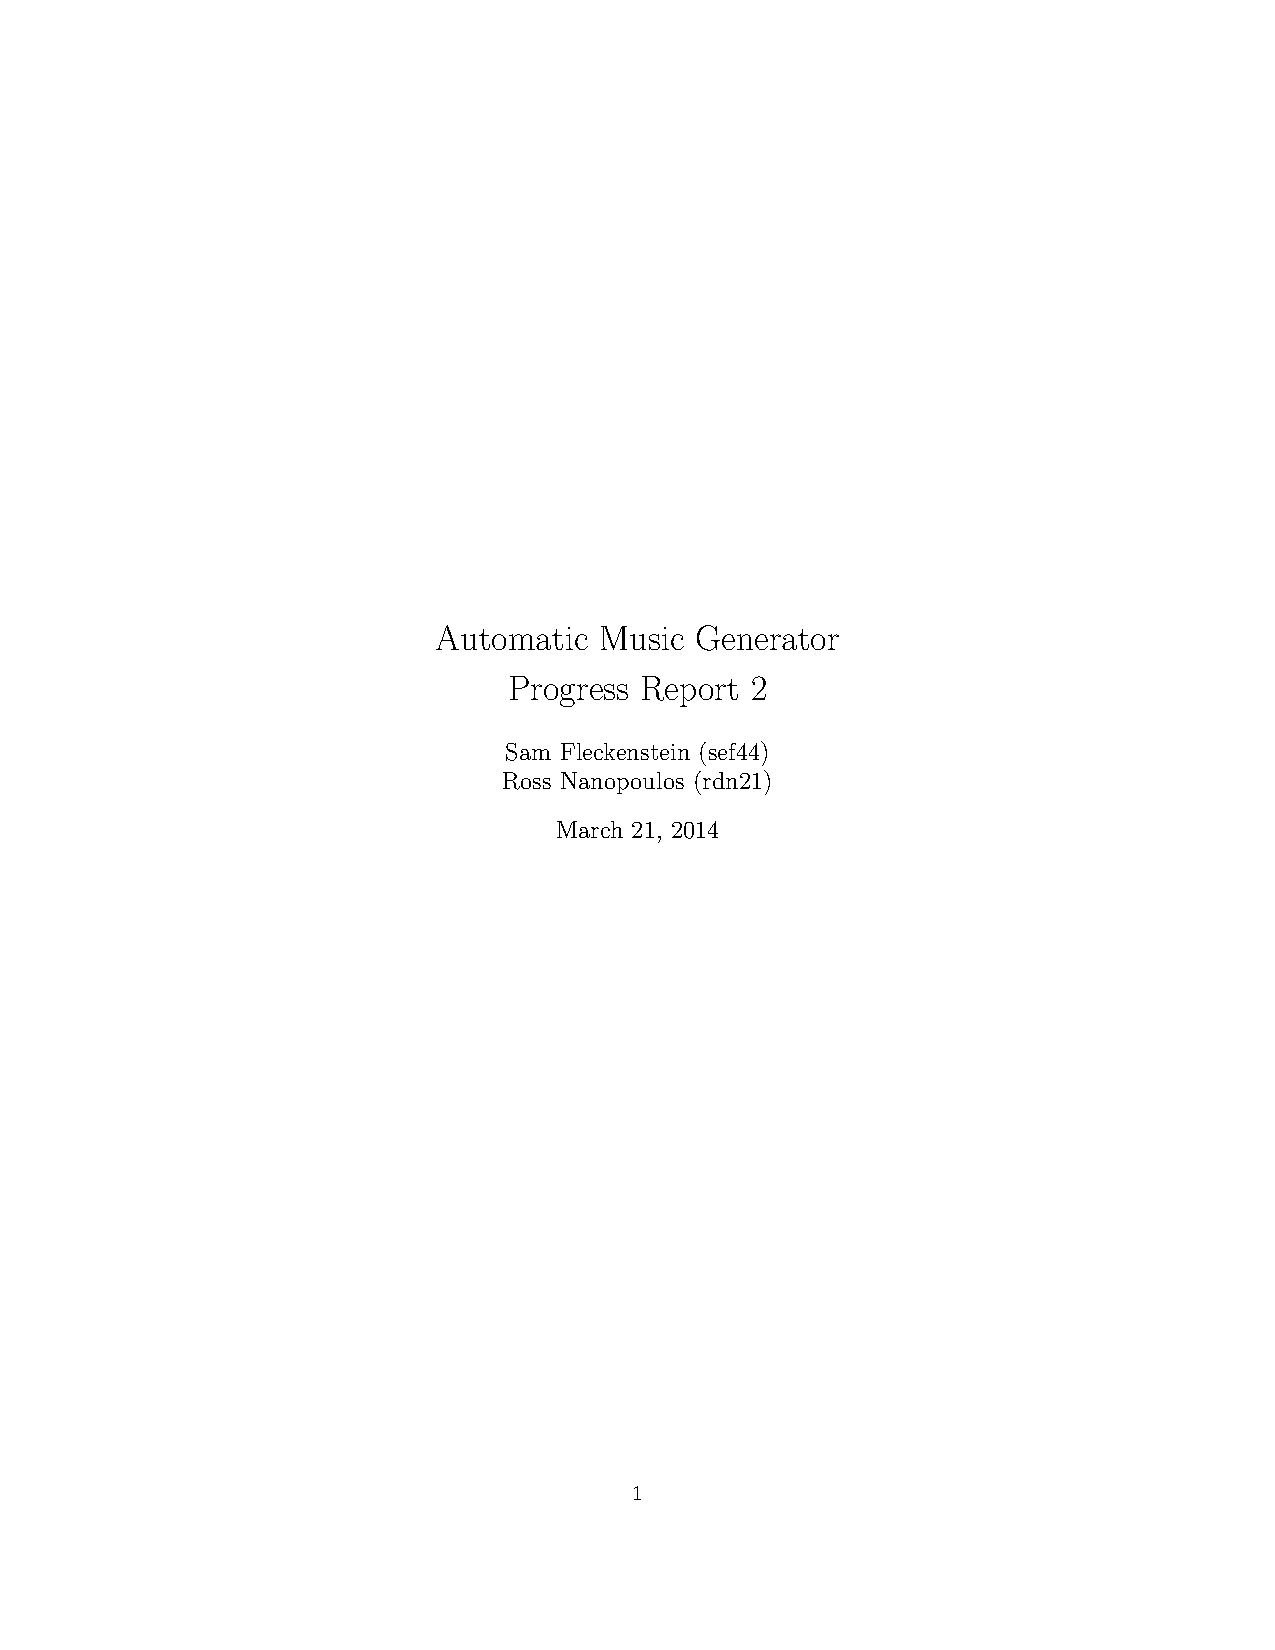
\includepdf[pages=-]{ProgressReport2.pdf}

\end{document}
